\documentclass[a4paper, 12pt]{report}

\usepackage{graphicx}

\begin{document}

% Title
\title{First assignment documentation}
% Author
\author{Le Minh Nghia - AAOGMU}
\maketitle
\pagenumbering{Roman}
% Table of contents:
\tableofcontents

%CHAPTER:
\chapter{Assignment's description}
\pagenumbering{arabic}
	Simulate a simplified Capitaly game. There are some players with different strategies, and a
cyclical board with several fields. Players can move around the board, by moving forward with
the amount they rolled with a dice. A field can be a property, service, or lucky field.
A property can be bought for 1000, and stepping on it the next time the player can build a house
on it for 4000. If a player steps on a property field which is owned by somebody else, the player
should pay to the owner 500, if there is no house on the field, or 2000, if there is a house on it.
Stepping on a service field, the player should pay to the bank (the amount of money is a
parameter of the field). Stepping on a lucky field, the player gets some money (the amount is
defined as a parameter of the field). There are three different kind of strategies exist. Initially,
every player has 10000.

\textbf{Greedy player}: If he steps on an unowned property, or his own property without a house, he
starts buying it, if he has enough money for it.

\textbf{Careful player}: he buys in a round only for at most half the amount of his money.

\textbf{Tactical player}: he skips each second chance when he could buy.

If a player has to pay, but he runs out of money because of this, he loses. In this case, his
properties are lost, and become free to buy.

Read the parameters of the game from a text file. This file defines the number of fields, and then
defines them. We know about all fields: the type. If a field is a service or lucky field, the cost of it
is also defined. After the these parameters, the file tells the number of the players, and then
enumerates the players with their names and strategies.

In order to prepare the program for testing, make it possible to the program to read the roll dices
from the file.

\textbf{Print out which player won the game, and how rich he is (balance, owned properties)}

%CHAPTER:
\chapter{Usage}

The input will be read from \textit{"assignments-1-input.txt"} which is placed in side the project folder. After running the Main, the winner of the game will be write to the console.

The input file defines the number of fields, and then defines them. We know about all fields: the type. If a field is a service or lucky field, the cost of it is also defined. After the these parameters, the file tells the number of the players, and then enumerates the players with their names and strategies.

For testing purpose, one can also put the roll dices in each turn at the end of the input file (these numbers can only be {1, 2, 3, 4, 5, 6}).

%CHAPTER:
\chapter{UML Diagram}
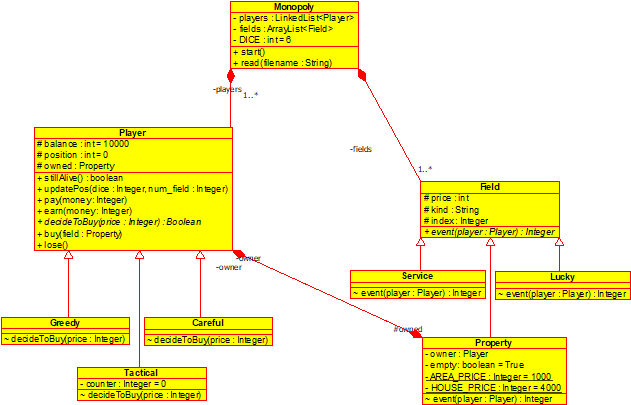
\includegraphics[scale=1.0]{classdiagram.png}

%CHAPTER:
\chapter{Methods documentation}
\begin{itemize}
\item \textbf{Monopoly's methods:}
		\begin{description}
			\item[start] Starts the game with list of players and list of fields and keep playing until only one player left, then output that player as the winner of the game.
			\item[read] Reads and stores the data from file.
		\end{description}
\item \textbf{Player's methods:}
		\begin{description}
			\item[stillAlive] Determines whether the player went bankrupt or not.
			\item[updatePos] Updates the current position of the player after rolling dice.
			\item[pay] Decreases player's balance by a given amount.
			\item[earn] Increases player's balance by a given amount.
			\item[decideToBuy] The decision of a player when stepped on an empty property or his owned property but haven not built a house yet. This is an abstract method and it will vary depending on the strategy.
				\begin{description}
					\item[Careful] Buys if the price does not exceed half of his money.
					\item[Greedy] Buys whenever he has a chance.
					\item[Tactical] Skips each second chance when he could buy.
				\end{description}
			\item[buy] The process of spending money for buying/building.
			\item[lose] Gives back all of his properties after losing.
		\end{description}
\newpage
\item \textbf{Field's methods:}
		\begin{description}
			\item[event] The event when a player stepped on the field. This is an abstract method and it will vary depending on the type of field and the decision of the player.
				\begin{description}
					\item[Lucky] The player earns some money.
					\item[Property] If the field is empty or the player who stepped on is the owner of the field, then he will decide to buy/upgrade the field. Else the player must pay the stepping fee to the owner.
					\item[Service] The player pays some money.
				\end{description}
		\end{description}
\end{itemize}

%CHAPTER:
\chapter{Testing}
%10 Tests.
\begin{enumerate}
\item
	\begin{itemize}
		\item Input
		
7

Service 5000

Service 4000

Service 3000

Lucky 233

Property

Property

Property

4

A Careful

B Greedy

C Tactical

D Tactical

1 4 3 1 5 6 3 2 1 5 1 6 4 2 4 4 6 3 6 6 3 2 5 2 3 2 6

		\item Output
		
B

Balance: 2199

Properties: [4]

	\end{itemize}
\item
	\begin{itemize}
		\item Input
		
7

Service 5000

Service 4000

Service 3000

Lucky 233

Property

Property

Property

4

A Careful

B Greedy

C Tactical

D Tactical

4 5 6 3 3 2 1 5 4 5 6 4 3 6 1 1 4

		\item Output
		
D

Balance: 3233

Properties: [6]

	\end{itemize}
\item
	\begin{itemize}
		\item Input

7

Property

Property

Property

Property

Property

Property

Property

4

A Careful

B Greedy

C Tactical

D Tactical

1 2 2 2 1 1 1 1 1 1 1 1 1 1 1 1 1 1 1 1 1 1 1 1 3 2 2 2 1 1 1 1 1 1 1 1 1 1 1 1 4 3 1 1 1

		\item Output
		
B

Balance: 17000

Properties: [2, 3, 4, 5, 6, 0]

	\end{itemize}
\item
	\begin{itemize}
		\item Input
		
7

Property

Property

Property

Property

Property

Property

Property

4

A Careful

B Greedy

C Tactical

D Tactical

1 2 2 2 1 1 1 1 1 1 1 1 1 1 1 1 1 1 1 1 1 1 1 1 3 2 2 2 1 1 1 1 1 1 1 1 1 1 1 1

		\item Output
		
Error in testing: Not enough turns to find the winner

	\end{itemize}
\item
	\begin{itemize}
		\item Input
		
-7

Property

Property

Property

Property

Property

Property

Property

4

A Careful

B Greedy

C Tactical

D Tactical

1 2 2 2 1 1 1 1 1 1 1 1 1 1 1 1 1 1 1 1 1 1 1 1 3 2 2 2 1 1 1 1 1 1 1 1 1 1 1 1 4 3 1 1 1

		\item Output
		
The input should not have negative numbers!

	\end{itemize}
\item
	\begin{itemize}
		\item Input

7

Service 5000

Service 4000

Service 3000

Lucky -233

Property

Property

Property

4

A Careful

B Greedy

C Tactical

D Tactical

4 5 6 3 3 2 1 5 4 5 6 4 3 6 1 1 4

		\item Output
		
The input should not have negative numbers!

	\end{itemize}
\item
	\begin{itemize}
		\item Input
		
7

Service X

Service 4000

Service 3000

Lucky 233

Property

Property

Property

4

A Careful

B Greedy

C Tactical

D Tactical

4 5 6 3 3 2 1 5 4 5 6 4 3 6 1 1 4

		\item Output
		
Not enough elements or invalid input!

	\end{itemize}
\item
	\begin{itemize}
		\item Input
		
7

Service 5000

Service 4000

Service 3000

Lucky 233

Property

Property

Property

4

A Careful

B Greedy

C Taccal

D Tactical

4 5 6 3 3 2 1 5 4 5 6 4 3 6 1 1 4

		\item Output
		
Invalid input!

	\end{itemize}
\item
	\begin{itemize}
		\item Input
		
7

Lucky 233

Lucky 233

Lucky 233

Lucky 233

Lucky 233

Lucky 233

Lucky 233

4

A Careful

B Greedy

C Taccal

D Tactical

4 5 6 3 3 2 1 5 4 5 6 4 3 6 1 1 4

		\item Output
		
This input will cause infinite loop game!
	
	\end{itemize}
\item
	\begin{itemize}
		\item Input
		
0

4

A Careful

B Greedy

C Taccal

D Tactical

4 5 6 3 3 2 1 5 4 5 6 4 3 6 1 1 4

		\item Output
		
This input will cause infinite loop game!

	\end{itemize}
\item
	\begin{itemize}
		\item Input
		
7

Service 233

Service 233

Service 233

Service 233

Service 233

Service 233

Service 233

0

4 5 6 3 3 2 1 5 4 5 6 4 3 6 1 1 4

		\item Output
		
This input will cause infinite loop game!

	\end{itemize}
\item
	\begin{itemize}
		\item Input
			
			The input is too big to be pasted here, take a look at \textit{"test/12.txt"}
		\item Output
			
QA

Balance: 10832

Properties: [23, 45, 58, 93]
	\end{itemize}
\end{enumerate}

\end{document}

